\documentclass[../mathNotesPreamble]{subfiles}

\providecommand{\relscalefact}{1.4}
\begin{document}
\relscale{\relscalefact}
  \section{1.3: Rates of Change and Behavior of Graphs}

  \begin{defn*}[Rate of Change]
    A rate of change describes how an output quantity changes
    relative to the change in the input quantity. The units on a
    rate of change are ``output units per input units''.

    The \textbf{average rate of change} between two input values is
    the total change of the function values divided by the input
    values.
    \[\dfrac{\Delta y}{\Delta x}=\dfrac{f(x_2)-f(x_1)}{x_2-x_1}\]
  \end{defn*}

  \begin{ex*}
    Suppose the following table contains temperatures recorded
    through the day.
    \begin{center}
      \begin{tabular}{@{}l*{5}{>{\hspace*{5mm}}r}@{}} \toprule
        $h$ & 7 AM & 9 AM & 11 AM & 1 PM & 3 PM \\\midrule
        $T(h)$ & $78^\circ F$ & $81^\circ F$ & $87^\circ F$ & $93^\circ F$ & $98^\circ F$ \\\bottomrule
      \end{tabular}
    \end{center}
    Find the average rate of change between
    \begin{extasks}[after-item-skip=\stretch{1}](3)
      \task 7 AM and 9 AM
      \task 9 AM and 11 AM
      \task 7 AM and 3 PM
    \end{extasks}
    \vspace*{\stretch{1}}
  \end{ex*}
  \pagebreak

  \begin{ex*}
    Using the following graph, determine the average rate of change on the interval $\sbrkt{-1,2}$
    \begin{flushright}
      \smash{\raisebox{-\height}{
      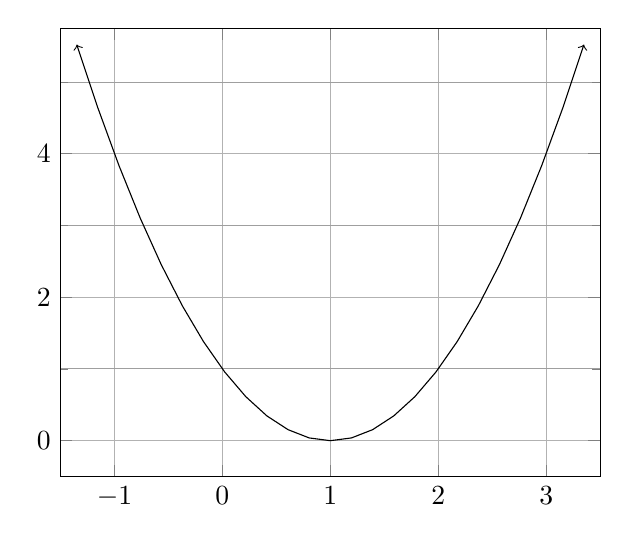
\begin{tikzpicture}[declare function={
        f(\x)=(\x-1)^2;}]
        \begin{axis}[
          grid=both, %major,minor
          grid style={line width=0.375pt, draw=gray!60},
          minor grid style={draw=gray!75},
          minor y tick num=1,
          xmin=-1.5, xmax=3.5,
          ymin=-0.5, ymax=5.75,
          ]
          \addplot[<->] expression[domain=-1.35:3.35]{f(x)};
        \end{axis}
      \end{tikzpicture}
      }}
    \end{flushright}
  \end{ex*}
  \vspace*{\stretch{1}}

  \begin{ex*}
    Find the average rate of change of $f(x)=x^2-\dfrac{1}{x}$ on the interval $\sbrkt{2,4}$.
  \end{ex*}
  \vspace*{\stretch{1}}
  \pagebreak

  \begin{ex*}
    Find the expression for the average rate of change of $g(t)=t^2+3t+1$ on the interval $\sbrkt{0,a}$.
  \end{ex*}
  \vspace*{\stretch{1}}

  \begin{defn*}
    Consider the function $f(x)$ on the interval $(a,b)$. Given \emph{any} two numbers $x_1$ and $x_2$ in $(a,b)$ where $x_1<x_2$, we say $f$ is
    \begin{center}
      \begin{tikzpicture}[declare function={
        a=1; b=2; c=3.4; d=1; ell=0.25; t=0.725; eps=0.05;
        f(\x)=(\x-a)*(\x-b)*(\x-c);
        lc(\x,\y,\ell)=(1-\ell)*\x+\ell*\y;
        quad_form(\a,\b,\c,\s)=(-\b+\s*sqrt(\b^2-4*\a*\c))/(2*\a);
        ap=quad_form(3,-2*(a+b+c), a*b+b*c+a*c,-1);
        bp=quad_form(3,-2*(a+b+c), a*b+b*c+a*c,1);
        xo=lc(a,b,t);     xt=lc(c,b,t);
        fo=f(xo);         ft=f(xt);
        xmin=lc(a,b,ell); xmax=lc(c,b,ell);
        ymin=d+f(bp)-eps; ymax=d-f(bp)+eps;
        }]
        \begin{groupplot}[
          group style={group size=2 by 1, horizontal sep=20mm},
          ymin=ymin, ymax=ymax,
          xtick={ap,xo,xt,bp}, xticklabels={$\vphantom{b}a$,$\vphantom{b}x_1$, $\vphantom{b}x_2$,$b$},
          yticklabels={$f(x_1)$, $f(x_2)$},
          xlabel=, ylabel=,
          ticklabel style={font=\normalsize,inner sep=0.5pt,fill=white,opacity=1.0, text opacity=1},
          every axis plot/.append style={domain=xmin:xmax,line width=0.95pt, color=lander_blue, samples=255},
          height=0.8*\axisdefaultheight,
          ]
            \nextgroupplot[ytick={d-fo,d-ft}, title=increasing if $f(x_1)<f(x_2)$]
              \addplot[<->] {d-f(x)};
              \addplot[soldot] coordinates{(xo,{d-f(xo)})(xt,{d-f(xt)})};
              \draw[dashed] (axis cs: xo,0) |- (axis cs: 0,d-fo)
                            (axis cs: xt,0) |- (axis cs: 0,d-ft);
            \nextgroupplot[ytick={d+fo,d+ft}, title=decreasing if $f(x_1)>f(x_2)$]
              \addplot[<->] {d+f(x)};
              \addplot[soldot] coordinates{(xo,{d+f(xo)})(xt,{d+f(xt)})};
              \draw[dashed] (axis cs: xo,0) |- (axis cs: 0,d+fo)
                            (axis cs: xt,0) |- (axis cs: 0,d+ft);
        \end{groupplot}
      \end{tikzpicture}
    \end{center}
  \end{defn*}
  \pagebreak

  \begin{defn*}[Relative/Local Extrema]
    A function $f$ has a
    \begin{itemize}
      \item
        \textbf{relative maximum} at $x=c$ if $f(c)\geq f(x)$ for every $x$ in $(a,b)$
      \item
        \textbf{relative minimum} at $x=c$ if $f(c)\leq f(x)$ for every $x$ in $(a,b)$
    \end{itemize}
  \end{defn*}
  \vspace*{\baselineskip}

  \begin{center}
    \begin{tikzpicture}[
      declare function={
        cubeRoot(\x)=\x/abs(\x)*abs(\x)^(1/3);
        f(\x)=\x<=7.81901? -(\x-6.81901)^7+1: 1.5*cubeRoot(\x-7.81901);},
      custNode/.style={
        align=center,
        color=black,
        inner sep=0.5pt,
        fill=white,
        opacity=0.95,
        text opacity=1},
      boxedNode/.style={
        custNode,
        rectangle,
        draw=black,
        rounded corners,
        inner sep=3pt
      }]
      \begin{axis}[
        axis lines=center,
        axis line style={black,->},
        xtick={1,2.7,3.87,4.9,5.55,6.81901,7.81901},
        xticklabels={,,,,,,},
        ymajorticks=false,
        xlabel=,ylabel=,
        height=\axisdefaultheight, width=0.95\linewidth,
        enlargelimits={value=0.025, auto},
%        ticklabel style={font=\footnotesize,inner sep=0.5pt,fill=white,opacity=1.0, text opacity=1},
        every axis plot/.append style={line width=0.95pt, color=lander_blue, samples=255},
        clip=false,
        ]
        \addplot[<->, smooth, tension=0.85] coordinates{(-0.25,-1)(0.25,0.75)(1,4)(2.5,1)(4,2)(5,-1)(5.5,5)};
        \addplot[<->] expression[domain=5.6:9] {f(x)};

        \draw[black, dashed] (axis cs: 1,0) -- (axis cs: 1,4);
        \draw[black, dashed] (axis cs: 2.7,0) -- (axis cs: 2.7,0.95);
        \draw[black, dashed] (axis cs: 3.87,0) -- (axis cs: 3.87,2);
        \draw[black, dashed] (axis cs: 4.9,0) -- (axis cs: 4.9,-1);
        \draw[black, dashed] (axis cs: 6.81901,0) -- (axis cs: 6.81901,1);

%        \draw[black, dashed] (axis cs: 5.55,-1.4) -- (axis cs: 5.55,5);
        \node[boxedNode, above, yshift= 5pt] at (1,4)         {relative\\max};
        \node[boxedNode, below, yshift=-10pt] at (2.7,-1)     {relative\\min};
        \node[boxedNode, above, yshift= 5pt] at (3.87,2.1)    {relative\\max};
        \node[boxedNode, below, yshift=-10pt] at (4.9,-1)     {relative\\min};
        \node[boxedNode, below, yshift=-10pt] at (7.81901,-1) {relative\\min};

        \node[custNode, below, yshift=-5pt] at (0.5,0)      {\textbf{inc}};
        \node[custNode, below, yshift=-5pt] at (1.85,0)     {\textbf{dec}};
        \node[custNode, below, yshift=-5pt] at (3.285,0)    {\textbf{inc}};
        \node[custNode, below, yshift=-5pt] at (4.35,0)     {\textbf{dec}};
        \node[custNode, below, yshift=-5pt] at (5.225,0)    {\textbf{inc}};
        \node[custNode, below, yshift=-5pt] at (6.184505,0) {\textbf{dec}};
        \node[custNode, below, yshift=-5pt] at (7.31901,0)  {\textbf{dec}};
        \node[custNode, below, yshift=-5pt] at (8.75,0)     {\textbf{inc}};
      \end{axis}
    \end{tikzpicture}
  \end{center}
  \vspace*{\stretch{1}}

  \begin{defn*}[Absolute Extrema]
    A function $f$ defined on a domain $D$ has an
    \begin{itemize}
      \item
        \textbf{absolute maximum} at $x=c$ if $f(c)\geq f(x)$ for every $x$ in $D$
      \item
        \textbf{absolute minimum} at $x=c$ if $f(c)\leq f(x)$ for every $x$ in $D$
    \end{itemize}
  \end{defn*}
  \pagebreak

  \begin{ex*}
    Using the following graph, find any relative and absolute extrema.
    \begin{flushright}
      \smash{\raisebox{-\height}{
      \begin{tikzpicture}[declare function={
        f(\x)=(\x)^2-2;}]
        \begin{axis}[
          grid=both, %major,minor
          grid style={line width=0.375pt, draw=gray!60},
          minor grid style={draw=gray!75},
          xmin=-2.5, xmax=2.5,
          ymin=-2.75, ymax=2.75,
          ]
          \addplot[-] expression[domain=-1:2]{f(x)};
          \addplot[soldot] coordinates{(-1,{f(-1)})(2,{f(2)})};
        \end{axis}
      \end{tikzpicture}
      }}
    \end{flushright}
  \end{ex*}
  \vspace*{\stretch{1}}
  \pagebreak

\end{document}
